\chapter{Przedstawienie problemu}

\section{Drzewa decyzyjne}

Podejmowanie decyzji jest procesem myślowym, który od początku istnienia ludzkości stwarza pewne trudności, a polega on na wybraniu najlepszego rozwiązania z dostępnych. Wpływ na optymalną decyzję mają informacje, które zostaną poddane analizie, ale także sama metoda analizy. Racjonalny wybór może być wspomagany różnymi algorytmami, czy też wizualną reprezentacją możliwych decyzji w postaci diagramu. Sam diagram może przybrać formę graficzną drzewa decyzyjnego.

Podstawowymi elementami drzewa są korzeń, gałęzie, węzły oraz liście. Korzeniem jest decyzja od którego rozpoczyna się budowa całej struktury zawierającej poszczególne węzły odpowiadające za sprawdzenie pewnego warunku. Natomiast gałęzie pełnią rolę połączenia wszystkich elementów \cite{misc_1}.  Liście są krańcowymi wierzchołkami drzewa i określają wybraną decyzje. Podczas próby określenia decyzji, należy poddać klasyfikacji posiadane dane, aby to osiągnąć konieczne jest przejście całego drzewa od samego korzenia do wynikowego liścia. Rezultatem takiej operacji będzie klasa definiująca decyzję.

\section{Uczenie maszynowe}
W otaczającym nas świecie ilość informacji produkowanych przez otoczenie oraz zbieranych przez firmy czy instytucje nadal przewyższa ilość danych, które można przeanalizować z użyciem obecnych zasobów. W celu wyciągnięcia wniosków z takiej ilości danych wykorzystuje się liczne rozwiązania technologiczne. Dzięki zastosowaniu różnych algorytmów przetwarzania danych, klasyfikacji oraz predykcji programy komputerowe posiadają możliwość uczenia się. Kierunek nauki, który zajmuje się tą dziedziną nazywamy uczeniem maszynowym. W ciągu ostatnich dziesięciu lat entuzjazm związany z wykorzystywaniem tej technologi wzrósł gwałtownie i w dużej mierze 
zdominował przemysł, ale również przyczynił się do jej rozwoju \cite{book_1}. Uczenie maszynowe stanowi trzon wielu usług, serwisów i aplikacji. Pod względem technologicznym odpowiada za wyniki wyszukiwania w przeglądarkach, za rozpoznawanie mowy przez nasze telefony, ale także jest odpowiedzialne za prowadzenie autonomicznych samochodów.

\section{Drzewa decyzyjne w technikach uczenia maszynowego}

Drzewa decyzyjne stanowią jedne z bardziej wszechstronnych algorytmów w  dziedzinie uczenia maszynowego. Z jednej strony mogą być wykorzystywane w zadaniach z zakresu klasyfikacji, a z drugiej strony również odgrywają ważną rolę w regresji \cite{book_1}. Z ich pomocą możemy uzyskać potężne modele i narzędzia zdolne do uczenia się ze złożonych zbiorów danych. Dodatkowym atutem drzew jest możliwość wizualnego przedstawienia rozwiązania, które będzie zrozumiałe dla osób nie mających do czynienia z uczeniem maszynowym lub ze statystyką. Z racji wzrostu popularności tej technologi zwiększyły się nakłady pracy naukowej w celu osiągnięcia coraz to lepszych i bardziej optymalnych algorytmów pod względem wydajnościowym. 

\subsection{System GDT}
Pracownicy Politechniki Białostockiej również mają wkład w budowę takich rozwiązań. Autorski system GDT (\textit{Global Decision Trees}), który jest wykorzystywany w aplikacji inżynierskiej, służy do generowania modelu drzewa decyzyjnego na podstawie zbiorów wejściowych \cite{sgdt_1}. Ten system jest zaimplementowany w języku c++ oraz jest skompilowany do pliku wykonywalnego, aby umożliwić jego uruchomianie z poziomu konsoli systemu operacyjnego. Całe rozwiązanie jest unikalne, a głównym założeniem jest wykorzystanie algorytmów genetycznych. Z ich pomocą przestrzeń rozwiązań danego problemu jest większa niż w klasycznym podejściu, co skutkuje możliwością osiągnięcia dokładniejszych i lepszych wyników \cite{sgdt_2}. Metody pracy algorytmów genetycznych w dużej mierze odwzorowują działania samej natury \cite{book_2}. Podczas definiowania pracy algorytmu należy podać takie parametry jak wielkość populacji, prawdopodobieństwo mutacji czy też krzyżowania się danych osobników. Wartości tych parametrów i innych są określane w pliku konfiguracyjnym opartym o strukturę XML, który jest zarazem plikiem wejściowym do aplikacji GDT. System oprócz tego pliku wykorzystuje pliki z konkretnymi rozszerzeniami:
\begin{itemize}
	\item *.data - plik zawierający dane treningowe, 
	\item *.test - plik zawierający dane testowe,
	\item *.names - plik określających nazwy klas oraz rodzaj zmiennych.
\end{itemize}
Na podstawie tych danych aplikacja GDT może stworzyć model drzewa decyzyjnego, którego przedstawienie jest zapisywane w pliku tekstowym. 

\section{Istniejące rozwiązania}
Aktualnie na rynku znajduje się mała liczba rozwiązań oferujących tworzenie drzew decyzyjnych. Aplikacje, które można wyróżnić różnią się między sobą zakresem funkcjonalności. Rozwiązania internetowe głównie są nastawione na zarobek, ale oferują też darmowe wersje z pewnymi ograniczeniami. Istnieją też liczne rozwiązania dla programistów w postaci paczek możliwych dla każdego z popularniejszych języków. Takie biblioteki umożliwiają w prosty sposób stworzenie podstawowych modeli uczenia maszynowego w tym drzew decyzyjnych. Negatywną cechą takiego rozwiązania jest wymagana przynajmniej podstawowa wiedza z zakresu programowania. Dodatkowo chcąc osiągnąć bardzo wydajne modele trzeba dokładnie znać mechanizmy działające pod strukturą biblioteki. Występują również nie liczne rozwiązania desktopowe. W głównej mierze są one rozwijane przez uniwersytety. Do wykonania obliczeń wymagają dobrej jakości sprzętu komputerowego, który umożliwi optymalną moc obliczeniową.    

\begin{figure}[htb]
	\centering
	
\includegraphics[width=11cm]{grafika/smartdraw.eps}
	\caption{Strona główna aplikacji \textit{SmartDraw}.}
	\label{rys21_smartdraw}
\end{figure}

\begin{figure}[htb]
	\centering
	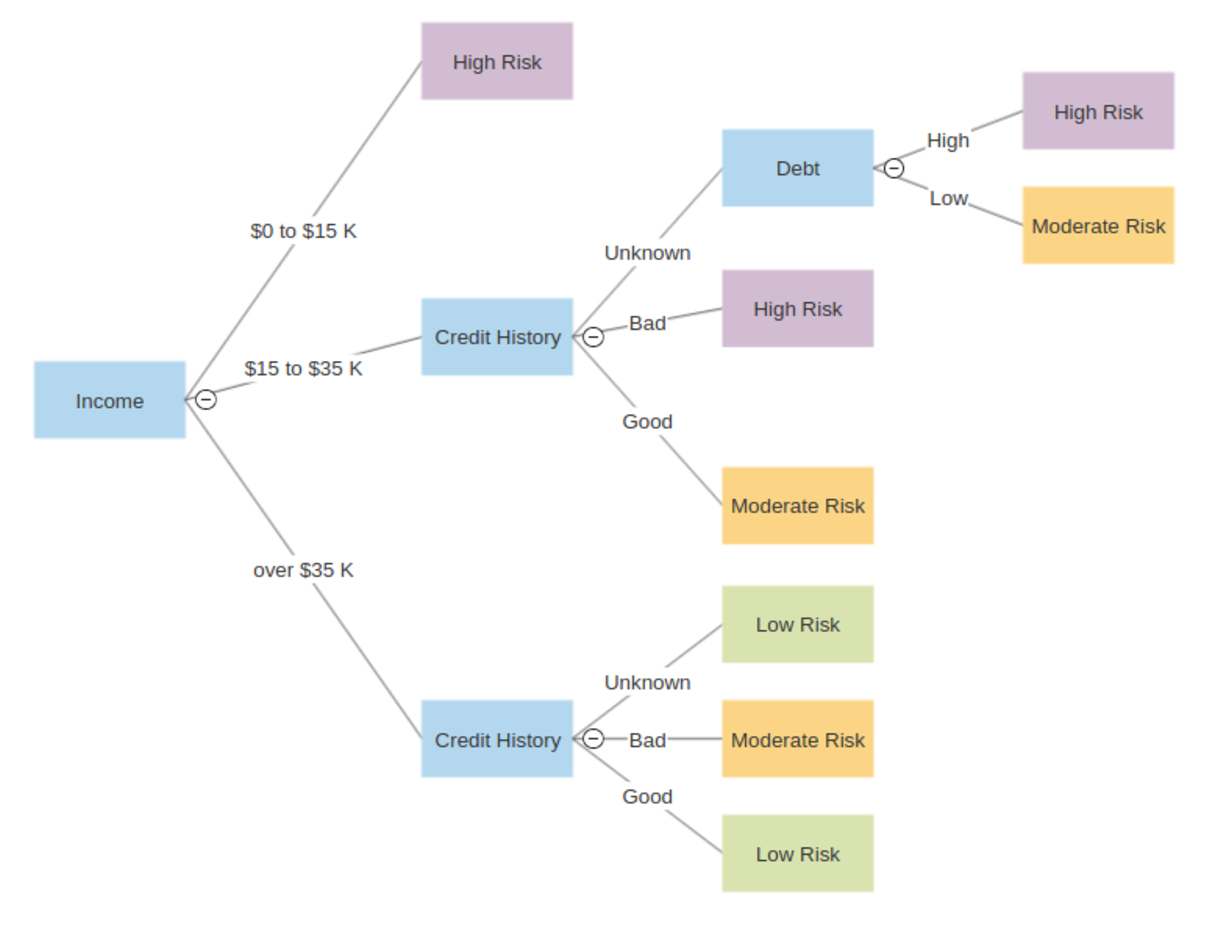
\includegraphics[width=11cm]{grafika/smartdraw_tree.eps}
	\caption{Drzewo stworzone w aplikacji \textit{SmartDraw}.}
	\label{rys22_smartdraw_tree}
\end{figure}


Aplikacja internetowa \textit{SmartDraw} jest jedną z wygodniejszych platform do tworzenia diagramów \cite{misc_smartdraw}. Dostęp do platformy następuje po przez przeglądarkę internetową. Założenie konta jest darmowe wraz z okresem próbnym. Po pewnym czasie aplikacja wymaga opłacenia miesięcznego abonamentu. Widok strony głównej został przedstawiony na Rys. \ref{rys21_smartdraw}. Platforma ponadto udostępnia funkcjonalność tworzenia innych rodzajów diagramów. Proces budowy nowego schematu przebiega po przez przeciągnie i łączenie bloków. Istnieje również możliwość wczytania struktury drzewa z pliku o rozszerzeniu *csv. Grafy są prezentowane w czytelny i przejrzysty sposób (Rys. \ref{rys22_smartdraw_tree}). Ukończony diagram można wyeksportować do pliku graficznego lub dokumentu programu Word. Aplikacja niestety nie umożliwia analizy informacji przy pomocy jakiegoś algorytmu. Skutkuje to brakiem opcji zbudowania drzewa decyzyjnego w pełni opartego o pliki ze zbiorami danych. 

\begin{figure}[htb]
	\centering
	
\includegraphics[width=11cm]{grafika/canva.eps}
	\caption{Strona główna aplikacji \textit{Canva}.}
	\label{rys23_canva}
\end{figure}

\begin{figure}[htb]
	\centering
	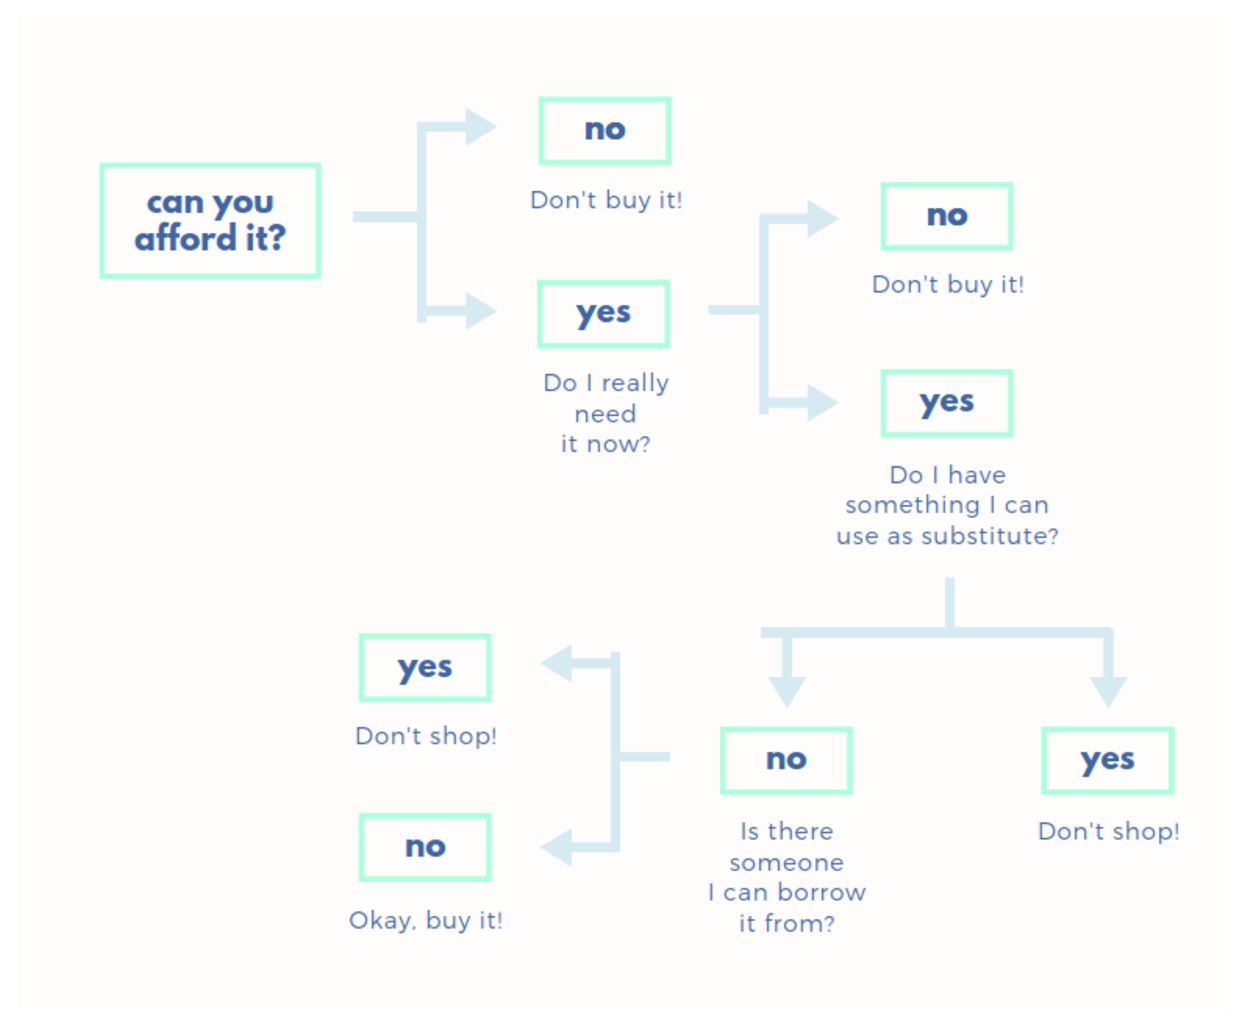
\includegraphics[width=11cm]{grafika/canvas_tree.eps}
	\caption{Drzewo stworzone w aplikacji \textit{Canva}.}
	\label{rys24_canva_tree}
\end{figure}

\textit{Canva} to kolejne narzędzie umożliwiające tworzenie drzew decyzyjnych przy pomocy przeglądarki internetowej \cite{misc_canva}. Dostęp do platformy wymaga założenia konta, które daje możliwość tworzenia projektów graficznych. Aplikacja posiada również rozszerzenia funkcjonalności przy pomocy pakietów płatnych dla firm, jak i osób prywatnych. Strona główna aplikacji została przedstawiona na Rys. \ref{rys23_canva}. Użytkownik ma możliwość tworzenia drzewa tylko poprzez przeciąganie konkretnych elementów. W aplikacji jednak brakuje opcji uzyskania drzewa na podstawie zbioru danych i wybranego algorytmu. Tworzone diagramy można wzbogacić o liczne walory wizualne i dostępne gotowe motywy (Rys. \ref{rys24_canva_tree}). Głównymi odbiorcami aplikacji są reklamodawcy oraz osoby prowadzące rozbudowaną działalność w serwisach społecznościowych.  
 
\begin{figure}[htb]
	\centering
	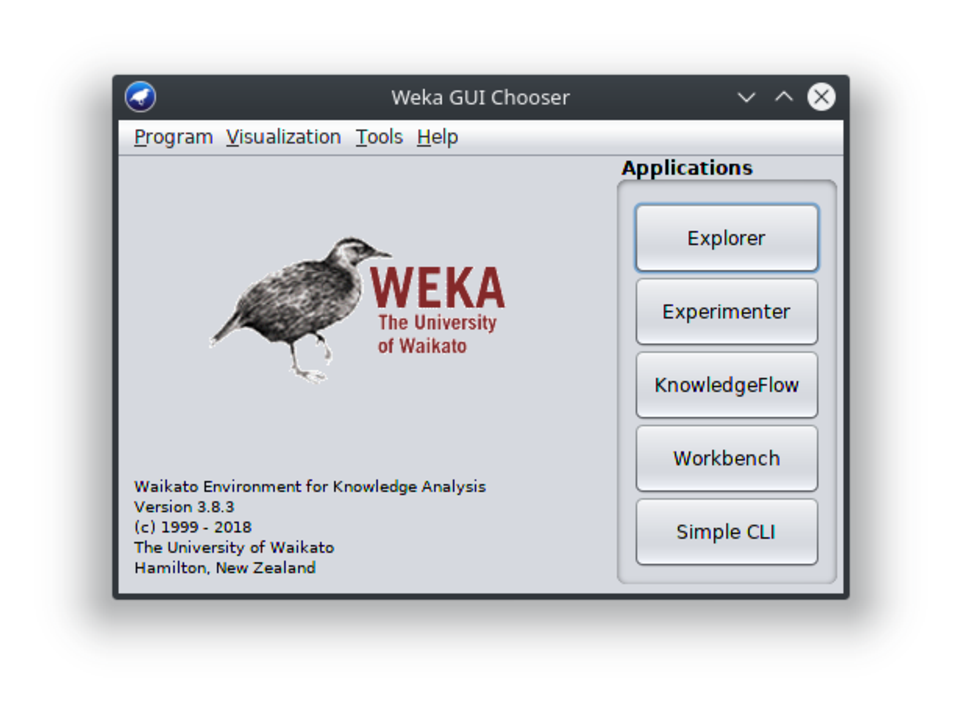
\includegraphics[height=7cm]{grafika/weka.eps}
	\caption{Okno główne aplikacji \textit{Weka}.}
	\label{rys25_weka}
\end{figure}

\begin{figure}[htb]
	\centering
	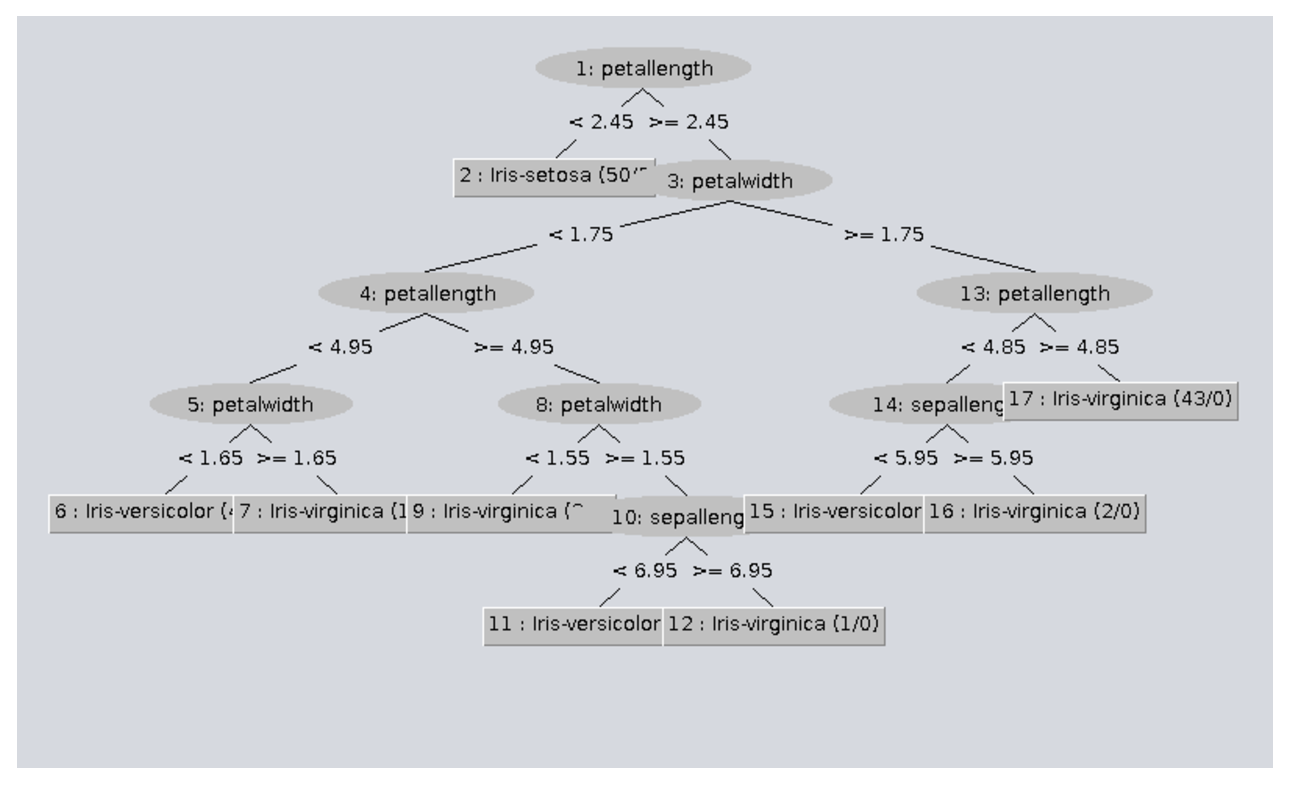
\includegraphics[width=11cm]{grafika/weka_tree.eps}
	\caption{Drzewo stworzone w aplikacji \textit{Weka}.}
	\label{rys26_weka_tree}
\end{figure}

\textit{Weka} jest narzędziem desktopowym stworzonym przez pracowników zajmujących się tematami uczenia maszynowego na Uniwersytecie Waikato w Nowej Zelandii. Aplikacja została zaimplementowana przy pomocy języka programowania Java. Dzięki temu platforma natywnie może działać na każdym systemie operacyjnym. Główne okno aplikacji zostało zaprezentowane na Rys. \ref{rys25_weka}. Posiada także liczne wrappery umożliwiające korzystanie z zaimplementowanych mechanizmów za pośrednictwem różnych języków programowania. Przy pomocy aplikacji użytkownika ma dostęp do dużej ilości algorytmów klasyfikacji z wykorzystaniem uczenia maszynowego, łącznie z drzewami decyzyjnymi. Tworzenie nowego eksperymentu zaczyna się od wybrania zestawu danych. Użytkownik początkujący może skorzystać z przykładowych plików. Po wczytaniu zbioru istnieje możliwość podejrzenia wizualizacji danych oraz ich wstępnej obróbka. W kolejnym kroku użytkownika musi wybrać interesujący go sposób klasyfikacji, do wyboru jest kilka różnych algorytmów związanych z tworzeniem drzew decyzyjnych, ale i nie tylko. Proces obliczeń potrwa pewien okres czasu i zależy głownie od ilości danych oraz zasobów mocy obliczeniowej. Rezultaty eksperymentu są przedstawione w postaci tekstowej, ale także istnieje opcja wyświetlenia grafu. Przykładowe drzewo decyzyjne stworzone za pośrednictwem programu zostało przedstawione na Rys. \ref{rys26_weka_tree}. Ponadto poszczególne atrybuty węzłów zostają zobrazowane za pośrednictwem wykresów. Aplikacja umożliwia również liczne modyfikacje w parametrach algorytmów mające na celu osiągniecie lepszych wyników.  

Rozwiązanie oferowane przez pracę dyplomową jest unikalne nie tylko ze względu na wykorzystany system GDT. Wyróżnia się w pełni niezależnością użytkownika od sprzętu, który posiada, co w przypadku takich rozwiązań jak program \textit{Weka} ma znaczenie. Aktualnie dostępne rozwiązania internetowe nie wyróżniają się miedzy sobą sposobem działania,a dodatkowo umożliwiają ograniczone funkcjonalności co do budowania drzew na podstawie zbiorów danych. Natomiast rozwiązania desktopowe wymagają od użytkownika dużej znajomości tego zagadnienia. Aplikacja powstała podczas pracy dyplomowej wypełnia lukę na rynku. Umożliwia darmowy, łatwy pod względem obsługi system dla użytkownika, nawet który dopiero zaczyna przygodę z uczeniem maszynowym. Co więcej rozszerza o takie funkcjonalności jak udostępnianie eksperymentów i przejrzysty sposób zarządzania nimi. 